% Technical document -- More than a Hack 2027, phase 1. Team MILF.
% Build: pdflatex MILF.tex (twice), or upload MILF.tex + fig/ to Overleaf (pdfLaTeX).
% Figures are produced by docs/paper/make_figures.py (aggregates only).
\documentclass[10pt,a4paper]{article}

\usepackage[T1]{fontenc}
\usepackage[utf8]{inputenc}
\usepackage{lmodern}
\usepackage[margin=2.1cm]{geometry}
\usepackage{microtype}
\usepackage{graphicx}
\usepackage{booktabs}
\usepackage{tabularx}
\usepackage{amsmath,amssymb}
\usepackage{xcolor}
\usepackage{enumitem}
\usepackage{caption}
\usepackage{float}
\usepackage{tikz}
\usetikzlibrary{arrows.meta,positioning,fit,calc}
\usepackage[hidelinks]{hyperref}
\usepackage{listings}

\definecolor{ink}{HTML}{0B0B0B}
\definecolor{ink2}{HTML}{52514E}
\definecolor{cH}{HTML}{2A78D6}
\definecolor{cA}{HTML}{EB6834}
\definecolor{cD}{HTML}{9A9993}
\definecolor{acc}{HTML}{1BAF7A}
\definecolor{codebg}{HTML}{F4F3F0}

\captionsetup{font=small,labelfont=bf}
\setlist{nosep,leftmargin=1.2em}
\setlength{\parskip}{3pt}
\lstset{basicstyle=\ttfamily\footnotesize,backgroundcolor=\color{codebg},frame=none,
        columns=fullflexible,breaklines=true,xleftmargin=4pt,aboveskip=4pt,belowskip=4pt}

\newcommand{\team}{MILF (Man I Love Ferm\'{\i}n)}
\newcommand{\members}{Tom\'as Cock, Jorge \'Angel, Samuel Botero}
\newcommand{\repourl}{\url{https://github.com/samulbm18/milf-more-than-a-hack-2027}}
\newcommand{\code}[1]{\texttt{#1}}
\newcommand{\lH}{\mathsf{H}}
\newcommand{\lA}{\mathsf{A}}
\newcommand{\lD}{\mathsf{D}}

\title{\vspace{-1.2cm}\textbf{Team ball possession from tracking data\\ as decoding of a football state machine}}
\author{Team \team\\[2pt]\small \members\\[2pt]
\small More than a Hack 2027, phase 1 --- FC Barcelona vs.\ Athletic Club\\
\small Code: \repourl}
\date{\small 17 November 2026}

\begin{document}
\maketitle
\vspace{-0.6cm}

%=====================================================================================================
\section{Approach}

The task is to assign each frame to home possession ($\lH$), away possession ($\lA$) or dead ball
($\lD$). The ranking metric, spellF1, scores possession spells rather than frames, so an output that
fluctuates between teams is penalised once per spurious spell even when frame accuracy is high. The
solution therefore separates two problems: \emph{detection} (local evidence about who controls the
ball and whether play is live) and \emph{decision} (a label sequence that is consistent with how a
match evolves). Detection is performed by a neural possession detector, a touch detector, stoppage
heuristics and the TV broadcast. Decision is made by a hidden semi-Markov model (HSMM) of the game,
decoded with Viterbi, followed by a small set of deterministic rules (Figure~\ref{fig:pipeline}).

\textbf{Why not a frame classifier.} An oracle analysis on the public window showed that the decoder
is not the bottleneck: given the true team on visible-ball steps, it reaches spellF1 0.92. A detector
that labels frames directly, however, converts its local errors into spurious turnovers. Treating
every detector as evidence and letting an explicit game model decide removes most of these
fluctuations and makes football constraints (persistence of possession, stoppages, restarts with a
clear possessor) part of the inference instead of post-hoc smoothing.

\begin{figure}[t]
\centering
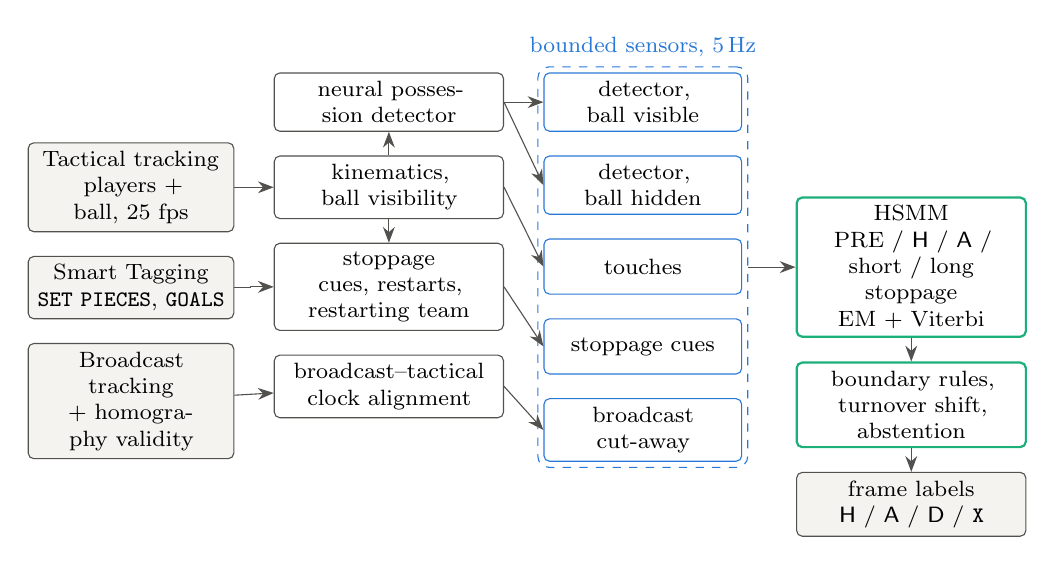
\begin{tikzpicture}[
  font=\footnotesize, node distance=3mm and 5mm,
  box/.style={draw=ink2, rounded corners=2pt, align=center, inner sep=3pt, minimum height=7mm, fill=white},
  data/.style={box, fill=codebg},
  sens/.style={box, draw=cH, text width=23mm},
  dec/.style={box, draw=acc, line width=0.8pt},
  ar/.style={-{Stealth[length=2mm]}, ink2}]
  \node[data, text width=24mm] (trk) {Tactical tracking\\ players + ball, 25 fps};
  \node[data, text width=24mm, below=of trk] (tag) {Smart Tagging\\ \code{SET PIECES}, \code{GOALS}};
  \node[data, text width=24mm, below=of tag] (bc) {Broadcast tracking\\ + homography validity};
  \node[box, right=of trk, text width=27mm] (frames) {kinematics, ball visibility};
  \node[box, below=of frames, text width=27mm] (events) {stoppage cues, restarts, restarting team};
  \node[box, below=of events, text width=27mm] (sync) {broadcast--tactical clock alignment};
  \node[box, above=of frames, text width=27mm] (net) {neural possession detector};
  \node[sens, right=of net] (s1) {detector, ball visible};
  \node[sens, below=of s1] (s2) {detector, ball hidden};
  \node[sens, below=of s2] (s3) {touches};
  \node[sens, below=of s3] (s4) {stoppage cues};
  \node[sens, below=of s4] (s5) {broadcast cut-away};
  \node[draw=cH, dashed, rounded corners, fit=(s1)(s5), inner sep=2pt, label={[cH]above:{bounded sensors, 5\,Hz}}] (S) {};
  \node[dec, right=6mm of S, text width=27mm] (hsmm) {HSMM\\ PRE / $\lH$ / $\lA$ /\\ short / long stoppage\\ EM + Viterbi};
  \node[dec, below=of hsmm, text width=27mm] (rules) {boundary rules, turnover shift, abstention};
  \node[data, below=of rules, text width=27mm] (csv) {frame labels\\ $\lH$ / $\lA$ / $\lD$ / \code{X}};
  \draw[ar] (trk) -- (frames);
  \draw[ar] (frames) -- (net);
  \draw[ar] (frames) -- (events);
  \draw[ar] (tag.east) -- ++(2mm,0) |- (events.west);
  \draw[ar] (bc) -- (sync);
  \draw[ar] (net.east) -- (s1.west);
  \draw[ar] (net.east) -- (s2.west);
  \draw[ar] (frames.east) -- (s3.west);
  \draw[ar] (events.east) -- (s4.west);
  \draw[ar] (sync.east) -- (s5.west);
  \draw[ar] (S.east) -- (hsmm.west);
  \draw[ar] (hsmm) -- (rules);
  \draw[ar] (rules) -- (csv);
\end{tikzpicture}
\caption{Overview. Detectors produce discrete observations; only the HSMM and the deterministic
boundary rules produce labels. Restarts and the restarting team parametrise transitions, not
observations.}
\label{fig:pipeline}
\end{figure}

\subsection{Game model}
Let $s_t$ be the hidden state at frame $t$ (25\,fps) and $o_t=(o_t^1,\dots,o_t^K)$ the discrete
symbols emitted by the $K$ detectors. The label sequence is the MAP state sequence
\begin{equation}
\hat s_{1:T}=\arg\max_{s_{1:T}} \; p(s_1)\prod_{t>1} p(s_t\mid s_{t-1}, t)\prod_{t}\prod_{k} E_k\!\left[\ell(s_t),o_t^k\right],
\end{equation}
where $\ell(s)\in\{\lH,\lA,\lD\}$ and $E_k[\ell,o]=P(o^k=o\mid\ell)$. Detectors are conditionally
independent given the label; a silent detector contributes a factor of one. The model runs at frame
resolution, but detectors emit only on every fifth frame (5\,Hz, one observation every 0.2\,s) and
are silent in between: consecutive frames carry almost the same information, and reading all of them
would count the same evidence five times and make every detector overconfident.

Per half, the states are PRE, $\lH$, $\lA$, short stoppage and long stoppage
(Figure~\ref{fig:machine}). Each state is expanded into a Coxian chain of phases, which yields
explicit duration distributions while inference remains exact and linear in the match length.
Prior mean durations are 3\,s for possessions and 15\,s and 60\,s for the two stoppage types. Two
transition families encode football knowledge:
\begin{itemize}
\item \textbf{Turnovers} $\lH\leftrightarrow\lA$ have probability proportional to $\tau\,b_t^{\,w_b}$
  ($w_b=2$), where $b_t$ is the turnover score of the neural detector. Changes of possession are
  concentrated where a local change is observed instead of following a constant hazard.
\item \textbf{Restarts} leave a stoppage towards $\lH$ with probability $\sigma(z_t)$ and towards
  $\lA$ with $1-\sigma(z_t)$, where $z_t$ is the restarting-team logit (Section~\ref{sec:rules}),
  and are only likely at detected restarts. Every restart thus has an explicit possessor.
\end{itemize}
Frames before each kick-off are the only hard constraints.

\begin{figure}[t]
\centering
\begin{minipage}[c]{0.50\linewidth}
\centering
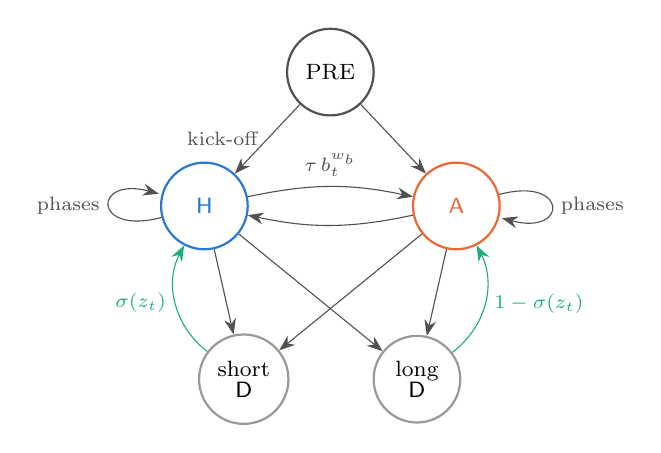
\begin{tikzpicture}[font=\footnotesize, >={Stealth[length=2mm]},
  st/.style={circle, draw, minimum size=11mm, align=center, line width=0.8pt},
  lab/.style={font=\scriptsize, ink2}]
  \node[st, draw=ink2] (pre) at (0,0) {PRE};
  \node[st, draw=cH, text=cH] (h) at (-1.6,-1.7) {$\lH$};
  \node[st, draw=cA, text=cA] (a) at (1.6,-1.7) {$\lA$};
  \node[st, draw=cD] (ds) at (-1.1,-3.9) {short\\[-2pt]$\lD$};
  \node[st, draw=cD] (dl) at (1.1,-3.9) {long\\[-2pt]$\lD$};
  \draw[->, ink2] (pre) -- node[lab, left]{kick-off} (h);
  \draw[->, ink2] (pre) -- (a);
  \draw[->, ink2, bend left=12] (h) to node[lab, above]{$\tau\, b_t^{w_b}$} (a);
  \draw[->, ink2, bend left=12] (a) to (h);
  \draw[->, ink2] (h) -- (ds); \draw[->, ink2] (h) -- (dl);
  \draw[->, ink2] (a) -- (ds); \draw[->, ink2] (a) -- (dl);
  \draw[->, acc, bend left=40] (ds) to node[lab, left, text=acc]{$\sigma(z_t)$} (h);
  \draw[->, acc, bend right=40] (dl) to node[lab, right, text=acc]{$1-\sigma(z_t)$} (a);
  \draw[->, ink2] (h) edge[loop left] node[lab]{phases} (h);
  \draw[->, ink2] (a) edge[loop right] node[lab]{phases} (a);
\end{tikzpicture}
\end{minipage}\hfill
\begin{minipage}[c]{0.46\linewidth}
\caption{State machine. Each state is a Coxian chain of phases (explicit durations). Turnovers are
modulated by the detector's turnover score $b_t$; restart edges (green; both stoppage types can
restart to either team) are weighted by the restarting-team probability $\sigma(z_t)$.}
\label{fig:machine}
\end{minipage}
\end{figure}

\subsection{Bounded sensors}\label{sec:obs}
Each detector is discretised into a few symbols. Its emission matrix is constrained in three ways:
\begin{enumerate}
\item \textbf{Team symmetry}: the $\lA$ row is the $\lH$ row with team symbols swapped.
\item \textbf{Bounded likelihood ratio}: $1/c\le E_k[\lH,o]/E_k[\lA,o]\le c$ with $c=4$ for every
  symbol, so that no single detector can outweigh the duration prior and the other sensors. A change
  of possession requires agreeing evidence. Compared with letting the neural detector decide, this
  improved spellF1 by $+0.025$ (better for 6 of 10 detector variants, equal for 1, worse for 3).
\item \textbf{Match-specific reliability}: matrices are re-estimated on the full match by EM
  (Baum--Welch, 3 iterations) as MAP estimates under a Dirichlet prior centred on the initial
  matrices, followed by the symmetry and ratio projections. No ground truth is involved.
\end{enumerate}
Table~\ref{tab:em} reports the learnt emissions of the non-neural sensors. The strongest
stoppage-heuristic level still occurs on 15\% of live steps, because the heuristics keep a stoppage
open until a restart kick is detected, often late; this is why heuristics are evidence, not rules.

\begin{table}[t]
\centering\small
\caption{Emission matrices after EM, $P(o\mid\ell)$; the $\lA$ row mirrors $\lH$.}
\label{tab:em}
\begin{tabular}{@{}l c ccc@{}}
\toprule
Sensor (symbols 0, 1, 2) & $\ell$ & 0 & 1 & 2\\
\midrule
touches (none, $\lH$ touch, $\lA$ touch) & $\lH$ & 0.706 & 0.227 & 0.067 \\
 & $\lD$ & 0.840 & 0.085 & 0.075 \\
\addlinespace
stoppage cues (none, weak, strong) & $\lH$ & 0.805 & 0.044 & 0.151 \\
 & $\lD$ & 0.309 & 0.171 & 0.520 \\
\addlinespace
broadcast (wide shot + ball, neither, cut-away) & $\lH$ & 0.847 & 0.150 & 0.003 \\
 & $\lD$ & 0.013 & 0.202 & 0.786 \\
\bottomrule
\end{tabular}
\end{table}

\subsection{Detectors}
\textbf{Neural possession detector.} A permutation-invariant set encoder over the player tokens and
the ball at each step, followed by a temporal transformer over 30\,s windows. It outputs
$q(\lH\mid t)$ on live play and the turnover score $b_t$; dead ball is deliberately not one of its
classes, since it is better observed by heuristics and the broadcast. Its initial targets are
rule-derived last-touch owners; it is then retrained once on the HSMM's own confident decisions
(posterior $\ge0.8$), which are more precise (owner precision 0.935 vs.\ 0.922) and cover occluded
intervals, so the detector absorbs the persistence and restart logic of the game model
($+0.071$ spellF1; a second round brought no gain).

\textbf{Touch detector and stoppage heuristics} implement the rules of Section~\ref{sec:rules}.

\textbf{Broadcast cut-aways.} The broadcast runs in real time through replays, so within each half
$t_{\text{tactical}}=t_{\text{broadcast}}+\Delta_h$. Both offsets are estimated automatically by FFT
cross-correlation of the two ball trajectories with a median refinement that is robust to replays
(residual 0.8\,m). When the broadcast leaves the wide shot (no valid pitch homography: replays,
close-ups) the ball is almost always dead. The director reacts 2--4\,s after play stops and returns
1--3\,s after it resumes, so the signal is advanced by 2.5\,s. On its own it identifies dead ball
with precision 0.97 and recall 0.87 on the public window. Its key property is independence from
tracking quality (Section~\ref{sec:missing}).

%=====================================================================================================
\section{Missing and noisy tracking}\label{sec:missing}
The ball is tracked on a median 57\% of frames per 5-minute block (minimum 20\%), against 88\% in the
public window (Figure~\ref{fig:vis}). The solution addresses this at the level of the model rather
than by imputing positions:
\begin{itemize}
\item \textbf{Visibility-dependent sensors.} The neural detector feeds two distinct sensors depending
  on whether the ball is tracked, because its reliability differs sharply: after EM,
  $P(\text{``$\lH$ sure''}\mid\lH)$ is 0.68 with the ball visible and 0.43 without. During occlusions
  the decision therefore rests on duration priors, restart evidence and the broadcast.
\item \textbf{Silence instead of negative evidence.} The touch sensor emits no symbol when the ball is
  not tracked, since a missing touch is not evidence of no touch. Suspected spare balls are treated as
  not visible.
\item \textbf{Robustness of the detector to gaps.} The neural detector is exposed to artificially
  hidden ball intervals during training, so that it infers control from the player configuration.
\item \textbf{An independent observation of stoppages.} Stoppages are hardest to detect where
  tracking is worst; broadcast cut-aways do not depend on tracking at all.
\end{itemize}
Using the broadcast ball as a substitute position was discarded: once aligned it covers only 12.6\%
of the frames where the tactical ball is missing.

\begin{figure}[t]
\centering
\includegraphics[width=\linewidth]{fig/visibility.pdf}
\caption{Share of frames with a tracked ball per 5-minute block. The public window (green) is the
easiest block of the match.}
\label{fig:vis}
\end{figure}

%=====================================================================================================
\section{Possession rules implemented}\label{sec:rules}
The rules act at three levels: as detector definitions, as transitions of the game model, and as
deterministic corrections of the decoded sequence.

\begin{description}[style=unboxed,leftmargin=0pt,itemsep=2pt]
\item[Touch.] A player is in contact with the ball when within 1.5\,m of it and either controls it
  (relative speed $\le3$\,m/s) or strikes it (ball acceleration peak $\ge18$\,m/s$^2$). Proximity
  alone would credit players running past the ball. Goalkeeper touches are not used as owner
  evidence, as they were the dominant source of wrong owners.
\item[Change of possession.] One touch confirms the current owner; a change requires a strike by the
  other team or 12 consecutive frames (0.48\,s) of contact. A deflection or a 50/50 duel does not
  transfer possession.
\item[Loose and contested balls.] There is no ``loose'' class: the ball stays with the last team in
  possession until the other team establishes control, since a loose-ball state would fragment
  possessions. The model places a turnover where evidence for the new team begins, i.e.\ when the
  ball leaves the old team, on average $\sim$0.43\,s before the reference; every direct
  $\lH\leftrightarrow\lA$ change is therefore shifted 10 frames later ($+0.020$ spellF1).
\item[Dead ball.] The ball is dead from the moment play stops until the restart. Stoppage cues
  (ball beyond a line by $>0.5$\,m; ball lost within 1.5\,m of a line while moving outward; still
  ball with frozen players for $\ge3$\,s; collective slowdown; \code{SET PIECES} tag; broadcast
  cut-away) are soft evidence with individual confidences, never hard constraints.
\item[Restart and restarting team.] Play resumes at the first kick (ball speed $>4$\,m/s for 3
  frames) after at least 1\,s of calm. The restarting team is a logit sum of the player nearest to the
  ball at the restart ($\pm2$), the team of a covering \code{SET PIECES} tag ($\pm1$) and, after a
  goal, the conceding team ($\pm3$). The out-of-play law (``the other team restarts'') agreed with the
  first touch after the restart only 50\% of the time, whereas the player at the ball is directly
  observed.
\item[Stoppage boundaries.] (i) A stoppage ending at most 6\,s before a tagged set piece is extended
  until 2\,s into the tag: the tag begins while the ball is still dead, but the broadcast has often
  returned to the wide shot, which the model reads as live play. (ii) A stoppage shorter than 2\,s is
  reassigned to the team in possession, since it would split one possession into two.
\item[Abstention.] Frames with maximum posterior below 0.75 are labelled \code{X} (3.4\% of graded
  frames). The scorer fills \code{X} with the previous label, so abstention is free when the previous
  label is correct and avoids committing to weakly supported turnovers ($+0.014$ to $+0.020$).
\end{description}

%=====================================================================================================
\section{Assets used and dropped}

\begin{table}[H]
\centering\small
\caption{Use of the provided assets.}
\label{tab:assets}
\begin{tabularx}{\linewidth}{@{}lXl@{}}
\toprule
Asset & Role & Status\\
\midrule
Tactical tracking & all observations & used\\
Smart Tagging \code{SET PIECES}, \code{GOALS} & stoppage cue, restarting team, boundary rule & used\\
Broadcast ball and homography validity & clock alignment; cut-away sensor & used\\
Broadcast ball as substitute ball position & fills only 12.6\% of tactical-ball gaps & dropped\\
Smart Tagging action codes as possession evidence & team tag agrees with the owner $\sim$50\% & dropped\\
Video & --- & not used\\
Public ground truth (5 min) & model selection only; never a training target & ---\\
\bottomrule
\end{tabularx}
\end{table}

Alternatives were compared \emph{paired}: the same detector outputs decoded with and without the
change, reporting the spellF1 difference and wins/ties/losses across detector variants
(Figure~\ref{fig:exp}). The most informative negative results:
\begin{itemize}
\item \textbf{Interception and pass-receiver logic}: no interception is detectable in the tracking at
  any of the 15 public turnovers, so turnovers cannot be localised from touches.
\item \textbf{Behavioural dead-ball classifier}: higher AUC than the heuristics (0.90 vs.\ 0.77), but
  its stoppages start 0.7\,s early and end 0.4\,s late, shortening adjacent possessions.
\item \textbf{Action tags as possession evidence}: their team field agrees with the owner only
  $\sim$50\% of the time ($-0.115$ to $0$).
\item \textbf{Reach-based control, trajectory-validated touches, restart geometry}: neutral.
\end{itemize}

\begin{figure}[t]
\centering
\includegraphics[width=\linewidth]{fig/experiments.pdf}
\caption{Paired $\Delta$ spellF1 of each alternative against the reference on the public window
(ranges where several settings were tested). Broadcast sensor and boundary rules are excluded:
they were assessed with whole-match criteria.}
\label{fig:exp}
\end{figure}

%=====================================================================================================
\section{Validation}\label{sec:results}
The public window allows only coarse conclusions: one possession is worth $\approx$0.02 spellF1 and
the bootstrap interval of the final score is 0.45--0.87. It also cannot reward better stoppages
(perfect stoppages give 0.645), because both public stoppages that are missed coincide with team
errors. The broadcast sensor and the boundary rules were therefore accepted on nine whole-match
consistency criteria whose thresholds were fixed before each variant was decoded
(Table~\ref{tab:match}).

\begin{figure}[t]
\centering
\includegraphics[width=\linewidth]{fig/ladder.pdf}
\caption{Cumulative contribution of each component, official evaluator on the public window.
Per-class F1 of the final system: $\lH$ 0.943, $\lA$ 0.908, $\lD$ 0.940 (dead-ball precision/recall
0.962/0.920, against 0.997/0.478 without the broadcast sensor).}
\label{fig:ladder}
\end{figure}

The bounded game model, the detector retraining, the turnover shift and abstention account for the
spellF1 gain (Figure~\ref{fig:ladder}). The broadcast sensor leaves public spellF1 unchanged but
raises macroF1 from 0.803 to 0.931 through dead-ball recall (0.478 $\to$ 0.920). Over the full match
the number of stoppages doubles, broadcast cut-aways falling inside a single predicted possession
drop from 37 to 1, and about 10 minutes of live play previously held as dead ball after late-detected
restarts are released (Figure~\ref{fig:strips}). Eight criteria are met; the ninth (set pieces with
dead ball in the 2\,s before the tag) proved mis-specified, as in quick restarts the tag begins when
play stops.

\begin{table}[H]
\centering\small
\caption{Whole-match consistency criteria (no ground truth).}
\label{tab:match}
\begin{tabular}{@{}lccc@{}}
\toprule
Criterion & No broadcast & + broadcast & \textbf{Final}\\
\midrule
Stoppages & 60 & 118 & \textbf{115}\\
Dead-ball share of graded frames & 0.314 & 0.422 & \textbf{0.428}\\
Possessions (per minute of play) & 211 (2.03) & 235 (2.26) & \textbf{235 (2.26)}\\
Cut-aways inside one predicted possession & 37 & 1 & \textbf{1}\\
Cut-aways across a team change without stoppage & 16 & 0 & \textbf{0}\\
Set pieces with $\lD$ in the 2\,s before the tag & 38/58 & 41/58 & \textbf{46/58}\\
Set pieces with a stoppage within 10\,s & 47/57 & 53/57 & \textbf{54/57}\\
Stoppages shorter than 2\,s & 1 & 4 & \textbf{0}\\
\bottomrule
\end{tabular}
\end{table}

\begin{figure}[t]
\centering
\includegraphics[width=\linewidth]{fig/public_strip.pdf}\\[2pt]
\includegraphics[width=\linewidth]{fig/match_strips.pdf}
\caption{Top: public window, ground truth against predictions (blue $\lH$, orange $\lA$, grey
$\lD$). Bottom: full match at 1\,s resolution without and with the broadcast sensor, together with
broadcast cut-aways and \code{SET PIECES} tags.}
\label{fig:strips}
\end{figure}

%=====================================================================================================
\section{Limitations}
\begin{itemize}
\item \textbf{Stoppage ends.} When the broadcast returns to the wide shot before an untagged restart
  (e.g.\ most free kicks), the stoppage ends early.
\item \textbf{Quick restarts.} Without a replay or an observed exit of the ball, a quick restart
  leaves no stoppage evidence (3 of 57 tagged set pieces).
\item \textbf{Short possessions.} 35\% of public possessions last under 4\,s versus 22\% of the
  predicted ones; transition F1 at $\pm1$\,s is 0.61. The touches that define these turnovers are
  mostly absent from the tracking.
\item \textbf{Generalisation.} Selection relied on five public minutes and unsupervised criteria; the
  private score is expected to be lower than the public one.
\end{itemize}
With more time: recovering the ball from video with a dedicated detector (it is missing on 43\% of
frames outside the public window), a small labelled live/dead validation set outside the public
window, and sharper behavioural stoppage boundaries.

%=====================================================================================================
\section{Reproduction}
Code: \repourl. The repository contains the source, pinned dependencies
(\code{requirements.lock}), installation instructions and the trained weights of the 12 detector
models; it contains no match data. With the challenge data bundle in \code{../more-than-a-hack-2027}
(or \code{MTAH\_ROOT}):
\begin{lstlisting}
python -m possession.pipeline --name MILF --rebuild --expect $(cat SUBMISSION.sha256)
\end{lstlisting}
The command rebuilds every intermediate file from the raw data, runs inference on the CPU in double
precision ($\sim$8 minutes, no GPU required), decodes, and fails unless the output matches the
submitted file (SHA-256 \code{b156296f\ldots7267}). The CPU path is the reference because
mixed-precision GPU inference changes a few hundred rows. PyTorch's fused attention path is disabled
at inference, since it otherwise converts additive attention biases into boolean masks. The weights
are part of the repository because GPU training is not deterministic: retraining from scratch
(\code{scripts/train\_from\_scratch.sh}, $\sim$3\,h on one GPU) yields an equivalent, not identical,
model.

\textbf{Verification.} \code{bash scripts/repro\_check.sh} copies only the files tracked by git into
an empty directory, rebuilds every cache from the raw data and runs the full pipeline. Run on the
published repository, it regenerated the submitted file byte for byte (SHA-256 \code{b156296f\ldots7267},
199\,319 rows), with the same public-window scores (spellF1 0.667, macroF1 0.931); the official
validator accepts the file and the 37 unit tests pass.

\end{document}
